% Unofficial University of Cambridge Poster Template
% https://github.com/andiac/gemini-cam
% a fork of https://github.com/anishathalye/gemini
% also refer to https://github.com/k4rtik/uchicago-poster

\documentclass[final]{beamer}

% ====================
% Packages
% ====================

\usepackage[T1]{fontenc}
\usepackage{lmodern}
\usepackage[orientation=portrait,size=a1,scale=1.2]{beamerposter}
\usetheme{gemini}
\usecolortheme{cam}
\usepackage{graphicx}
\usepackage{booktabs}
\usepackage[numbers]{natbib}
\usepackage{tikz}
\usepackage{pgfplots}
\pgfplotsset{compat=1.14}
\usepackage{anyfontsize}


\bibliographystyle{abbrvnat}
% ====================
% Lengths
% ====================

% If you have N columns, choose \sepwidth and \colwidth such that
% (N+1)*\sepwidth + N*\colwidth = \paperwidth
\newlength{\sepwidth}
\newlength{\colwidth}
\setlength{\sepwidth}{0.025\paperwidth}
\setlength{\colwidth}{0.5\paperwidth}

\newcommand{\separatorcolumn}{\begin{column}{\sepwidth}\end{column}}

% ====================
% Title
% ====================

\title{\huge A Survey of Explainable AI (XAI) Methods for Convolutional Neural Networks}

\author{\large Antonio Fernando Silva e Cruz Filho \inst{1} \and João Gabriel Andrade de Araujo Josephik\inst{1} \and Prof. Dr. Nina S. T. Hirata}

\institute[shortinst]{\inst{1} Institute of Mathematics and Statistics}

% ====================
% Footer (optional)
% ====================

\footercontent{
  \href{http://bit.ly/3V8BNdc}{http://bit.ly/3V8BNdc} \hfill
  Capstone Project - IME/USP \hfill
  fernandof.cruz@usp.br/joao.gabrielaaj@usp.br}
% (can be left out to remove footer)

% ====================
% Logo (optional)
% ====================

% use this to include logos on the left and/or right side of the header:
% \logoright{\includegraphics[height=7cm]{logo1.pdf}}
% \logoleft{\includegraphics[height=7cm]{logo2.pdf}}

% ====================
% Body
% ====================

\begin{document}

% Refer to https://github.com/k4rtik/uchicago-poster
% logo: https://www.cam.ac.uk/brand-resources/about-the-logo/logo-downloads
% \addtobeamertemplate{headline}{}
% {
%     \begin{tikzpicture}[remember picture,overlay]
%       \node [anchor=north west, inner sep=3cm] at ([xshift=0.0cm,yshift=1.0cm]current page.north west)
%       {\includegraphics[height=4.5cm]{logos/cambridge-reversed-color-logo.eps}}; 
%     \end{tikzpicture}
% }

% Acredito que podemos usar uma estrutura assim:

% Introduction
% Feature Visualization
% Saliency Maps
% LIME in Images
% Experiments
% Conclusion
% References

\begin{frame}[t]
\begin{columns}[t]
\separatorcolumn

\begin{column}{\colwidth}

  \begin{block}{Introduction}

    As artificial intelligence (AI) becomes part of critical fields like healthcare, finance, and autonomous vehicles, it’s important to understand how these systems make decisions. This is where Explainable AI (XAI) comes in. XAI helps make AI models, which are often complex, easier to understand and interpret. This ensures that AI systems are trusted and used responsibly.

    Neural networks are powerful tools for tasks like recognizing images or making predictions. However, they are often seen as "black boxes" because it’s hard to explain how they reach their decisions. This lack of clarity can be a problem in areas where understanding the reason behind a decision is as important as the result itself.
    \begin{columns}
      
      \begin{column}{0.6\textwidth}
        \begin{figure}
          \centering
          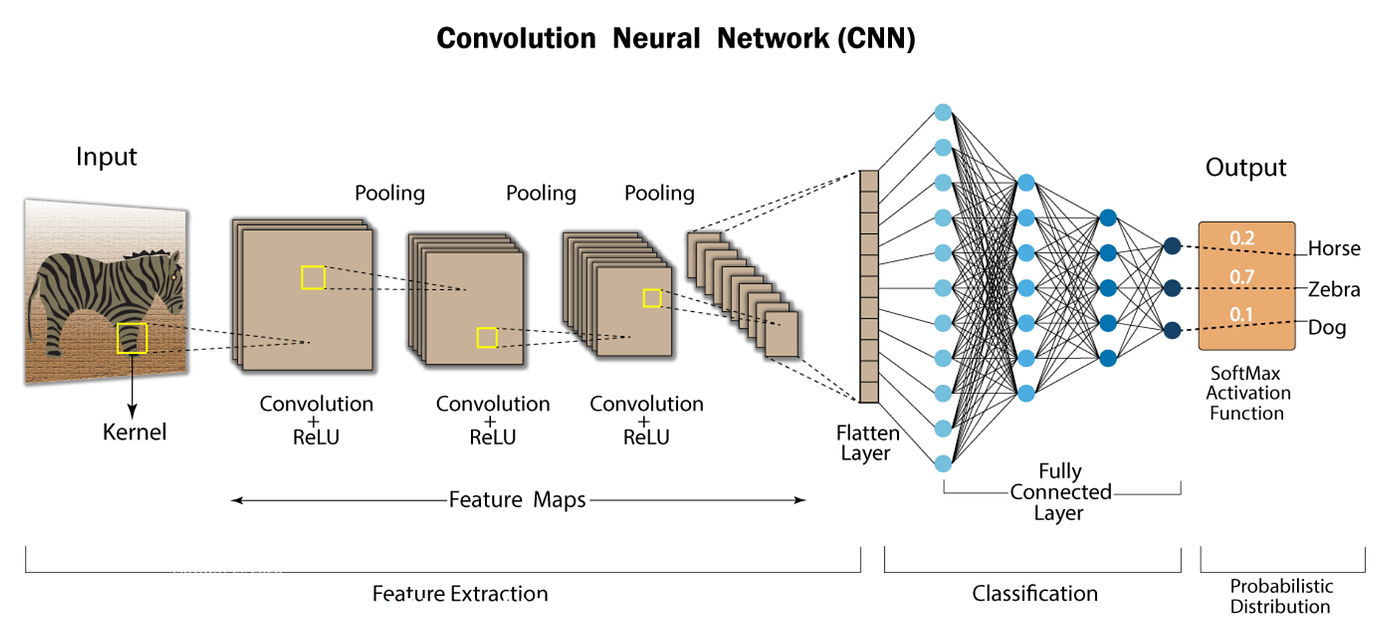
\includegraphics[width=\linewidth]{images/cnns.png}
          \caption{Convolutional Neural Network Architecture}
        \end{figure}
      \end{column}

      \begin{column}{0.4\textwidth}        
        
        \textbf{Convolutional Neural Networks (CNNs)} are neural networks designed for image and spatial data. They process parts of an image (like edges or textures) and combine these features to make decisions, making them ideal for tasks like face or object recognition.
        However, CNNs are also complex, and it can be hard to tell what they are focusing on and why. 
        XAI tools can help with this by showing how the CNN works step by step.
      \end{column}
    
    \end{columns}
    We will explore methods such as Feature Visualization, Saliency Maps, and LIME focused on explaining black-box image models like CNNs, aiming to create more robust, reliable, and less biased networks.
  \end{block}

  \begin{block}{Feature Visualization}
    CNNs can learn abstract features and concepts from images. 
    One can use techniques such as Feature Visualization to visualize the learned features by maximizing a network's neuron (or a set of neurons) value.
    This technique, called \emph{Activation Maximization}, can be modeled by the formula below, using the \emph{Gradient Ascent} method:
    \[x_{t + 1} = x_{t} + \mu \;\frac{\partial a(\theta, x_t)}{\partial x_t}\]
    Where \(x_t\) represents an image at iteration \(t\), \(\mu\) represents a tunable hyperparameter and the function \(a\) represents the forward pass of a unit in a Neural Network with parameters \(\theta\).
  \end{block}

  \begin{block}{Saliency Maps}

    GRADCAM OMG!!!!

  \end{block}

  \begin{alertblock}{A highlighted block}

    This block catches your eye, so \textbf{important stuff} should probably go
    here.

    Curabitur eu libero vehicula, cursus est fringilla, luctus est. Morbi
    consectetur mauris quam, at finibus elit auctor ac. Aliquam erat volutpat.
    Aenean at nisl ut ex ullamcorper eleifend et eu augue. Aenean quis velit
    tristique odio convallis ultrices a ac odio.
  \end{alertblock}

\end{column}

\separatorcolumn

\begin{column}{\colwidth}

  \begin{block}{LIME in Images}

    Vivamus congue volutpat elit non semper. Praesent molestie nec erat ac
    interdum. In quis suscipit erat. \textbf{Phasellus mauris felis, molestie
    ac pharetra quis}, tempus nec ante. Donec finibus ante vel purus mollis
    fermentum. Sed felis mi, pharetra eget nibh a, feugiat eleifend dolor. Nam
    mollis condimentum purus quis sodales. Nullam eu felis eu nulla eleifend
    bibendum nec eu lorem. Vivamus felis velit, volutpat ut facilisis ac,
    commodo in metus.

    \begin{enumerate}
      \item \textbf{Morbi mauris purus}, egestas at vehicula et, convallis
        accumsan orci. Orci varius natoque penatibus et magnis dis parturient
        montes, nascetur ridiculus mus.
      \item \textbf{Cras vehicula blandit urna ut maximus}. Aliquam blandit nec
        massa ac sollicitudin. Curabitur cursus, metus nec imperdiet bibendum,
        velit lectus faucibus dolor, quis gravida metus mauris gravida turpis.
      \item \textbf{Vestibulum et massa diam}. Phasellus fermentum augue non
        nulla accumsan, non rhoncus lectus condimentum.
    \end{enumerate}

  \end{block}

  \begin{block}{Experiments}

    Et rutrum ex euismod vel. Pellentesque ultricies, velit in fermentum
    vestibulum, lectus nisi pretium nibh, sit amet aliquam lectus augue vel
    velit. Suspendisse rhoncus massa porttitor augue feugiat molestie. Sed
    molestie ut orci nec malesuada. Sed ultricies feugiat est fringilla
    posuere.

\vspace{1em}

\begin{columns}
\begin{column}{0.4\textwidth}
\begin{center}
      \begin{figure}
      \begin{tikzpicture}
        \begin{axis}[
            scale only axis,
            no markers,
            domain=0:2*pi,
            samples=100,
            axis lines=center,
            axis line style={-},
            ticks=none]
          \addplot[red] {sin(deg(x))};
          \addplot[blue] {cos(deg(x))};
        \end{axis}
      \end{tikzpicture}
      \caption{Another figure caption.}
    \end{figure}
   \end{center}
\end{column}
\begin{column}{0.6\textwidth}  %%<--- here
\justify
Lorem ipsum dolor sit amet, consectetur adipiscing elit. Aliquam vel dapibus erat. Morbi quis leo congue, lobortis augue bibendum, malesuada neque. Duis ullamcorper quis orci sed consequat. Nam pellentesque ullamcorper tempor. Duis eget nulla blandit, vulputate orci vitae, ullamcorper ligula. Mauris a urna ac massa dignissim scelerisque sed et augue. Donec eget urna vitae neque elementum pellentesque et eget enim. Praesent a fermentum nibh. Nullam eu nibh neque. 
\end{column}
\end{columns}


  \end{block}

  \begin{block}{Conclusion}

    Nulla eget sem quam. Ut aliquam volutpat nisi vestibulum convallis. Nunc a
    lectus et eros facilisis hendrerit eu non urna. Interdum et malesuada fames
    ac ante \textit{ipsum primis} in faucibus. Etiam sit amet velit eget sem
    euismod tristique. Praesent enim erat, porta vel mattis sed, pharetra sed
    ipsum. Morbi commodo condimentum massa, \textit{tempus venenatis} massa
    hendrerit quis. Maecenas sed porta est. Praesent mollis interdum lectus,
    sit amet sollicitudin risus tincidunt non.

    Etiam sit amet tempus lorem, aliquet condimentum velit. Donec et nibh
    consequat, sagittis ex eget, dictum orci. Etiam quis semper ante. Ut eu
    mauris purus. Proin nec consectetur ligula. Mauris pretium molestie
    ullamcorper. Integer nisi neque, aliquet et odio non, sagittis porta justo.

    \begin{itemize}
      \item \textbf{Sed consequat} id ante vel efficitur. Praesent congue massa
        sed est scelerisque, elementum mollis augue iaculis.
        \begin{itemize}
          \item In sed est finibus, vulputate
            nunc gravida, pulvinar lorem. In maximus nunc dolor, sed auctor eros
            porttitor quis.
          \item Fusce ornare dignissim nisi. Nam sit amet risus vel lacus
            tempor tincidunt eu a arcu.
          \item Donec rhoncus vestibulum erat, quis aliquam leo
            gravida egestas.
        \end{itemize}
      \item \textbf{Sed luctus, elit sit amet} dictum maximus, diam dolor
        faucibus purus, sed lobortis justo erat id turpis.
      \item \textbf{Pellentesque facilisis dolor in leo} bibendum congue.
        Maecenas congue finibus justo, vitae eleifend urna facilisis at.
    \end{itemize}

  \end{block}

  \begin{block}{References}
    \nocite{*}
    \bibliography{bibliography}

  \end{block}

\end{column}

\end{columns}
\end{frame}

\end{document}
